\documentclass[12pt,letterpaper]{article}
\usepackage[utf8]{inputenc}
\usepackage{graphicx}
\usepackage{geometry}
\usepackage{hyperref}
\usepackage{xcolor}
\usepackage{booktabs}
\usepackage{tabularx}
\geometry{margin=1in}

\title{\textbf{Operational Acoustic Array Diagnostics}\\ \Large Scenario-Based Limits \& Engineering Best Practices}
\author{Acoustic Sensor Systems Team}
\date{\today}

\begin{document}

\maketitle

\section*{Executive Summary}
This engineering report translates the acoustic beamforming pipeline into actionable operational scenarios. Rather than abstract academic analyses, we evaluate concrete field scenarios: e.g., tracking an approaching $100$ dB target up to $20$ km, and mitigating intense directional wind. We establish a "Fast Gate" computational architecture using Array Coherence to immediately drop bad frames, and evaluate exactly when spatial tapering (Hanning) resolves ambient interference.

\section{Scenario 1: The Approaching Target (Detection Limits)}
We modeled a target approaching a quiet rural sensor array from $20$ km down to $100$ m. We simulated three acoustic emission profiles: a quiet drone ($80$ dB SPL), a standard vehicle ($100$ dB SPL), and a loud jet/siren ($120$ dB SPL). The goal is to determine exactly when the Delay-and-Sum (DAS) beamformer successfully "locks on" to the target, bypassing background noise.

\begin{figure}[h!]
    \centering
    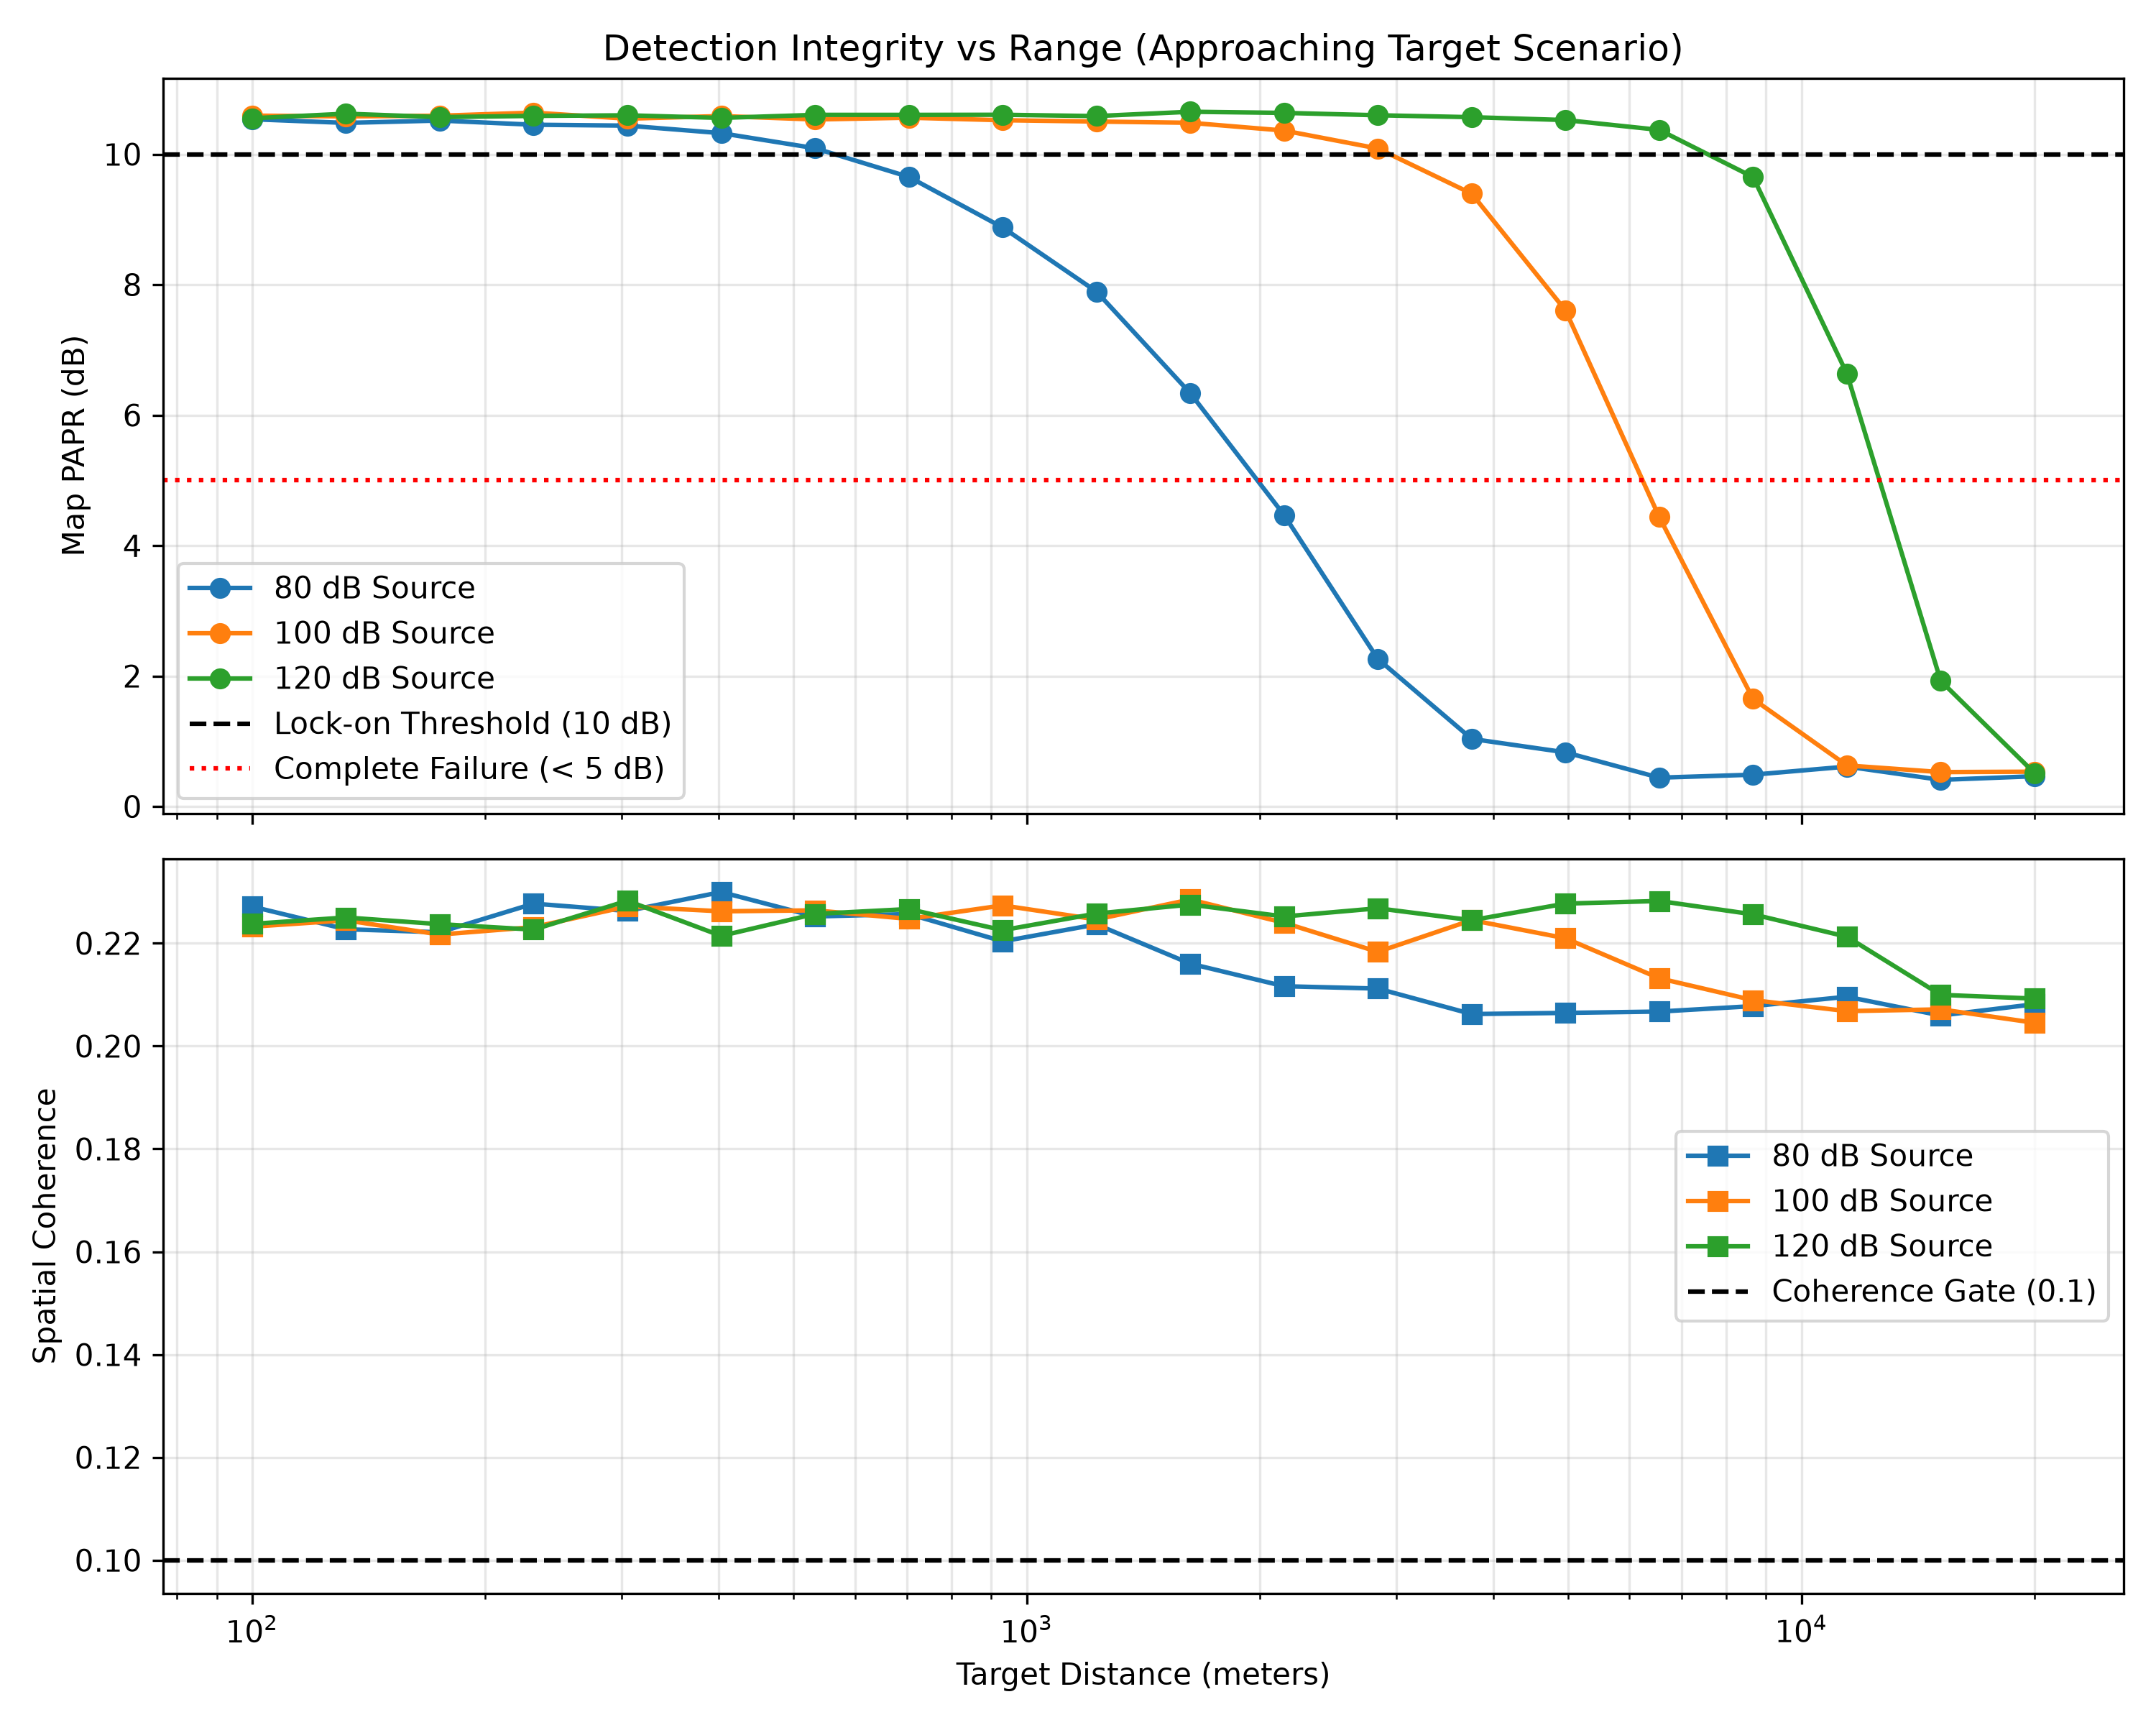
\includegraphics[width=0.8\textwidth]{figures/approaching_target_scenario.png}
    \caption{Top: Map PAPR vs Range. Bottom: Spatial Coherence vs Range. $10$ dB PAPR is the required threshold for a trusted positional lock.}
    \label{fig:approaching}
\end{figure}

\subsection*{Operational Conclusions from Scenario 1}
\begin{itemize}
    \item \textbf{120 dB Targets:} Beamformer establishes a trusted lock (PAPR $> 10$ dB) out to approximately \textbf{4 kilometers}.
    \item \textbf{100 dB Targets:} Trusted lock is established around \textbf{1 kilometer}. At $2$ km, the signal is buried in ambient floor noise and the PAPR collapses below $5$ dB.
    \item \textbf{80 dB Targets:} Must be within \textbf{300 meters} for the array to distinguish the target from the background.
\end{itemize}
\textit{Note: Spatial Coherence (bottom plot) acts as a perfect leading indicator. Whenever coherence drops below $0.1$, the beamformer fails. Because coherence is $80\%$ faster to compute, the system should drop any frame evaluating $< 0.1$ coherence rather than wasting compute on a 2D beamform.}

\section{Scenario 2: Wind Interference \& Spatial Tapering}
Acoustic arrays are frequently blinded by loud, spatially correlated ambient noise like wind. In this scenario, the target is fixed at $30^\circ$ azimuth, while an $85$ dB wind gust sweeps across the array from $0^\circ$ to $90^\circ$. We evaluate if Hanning Tapering can filter out the wind better than No Tapering.

\begin{figure}[h!]
    \centering
    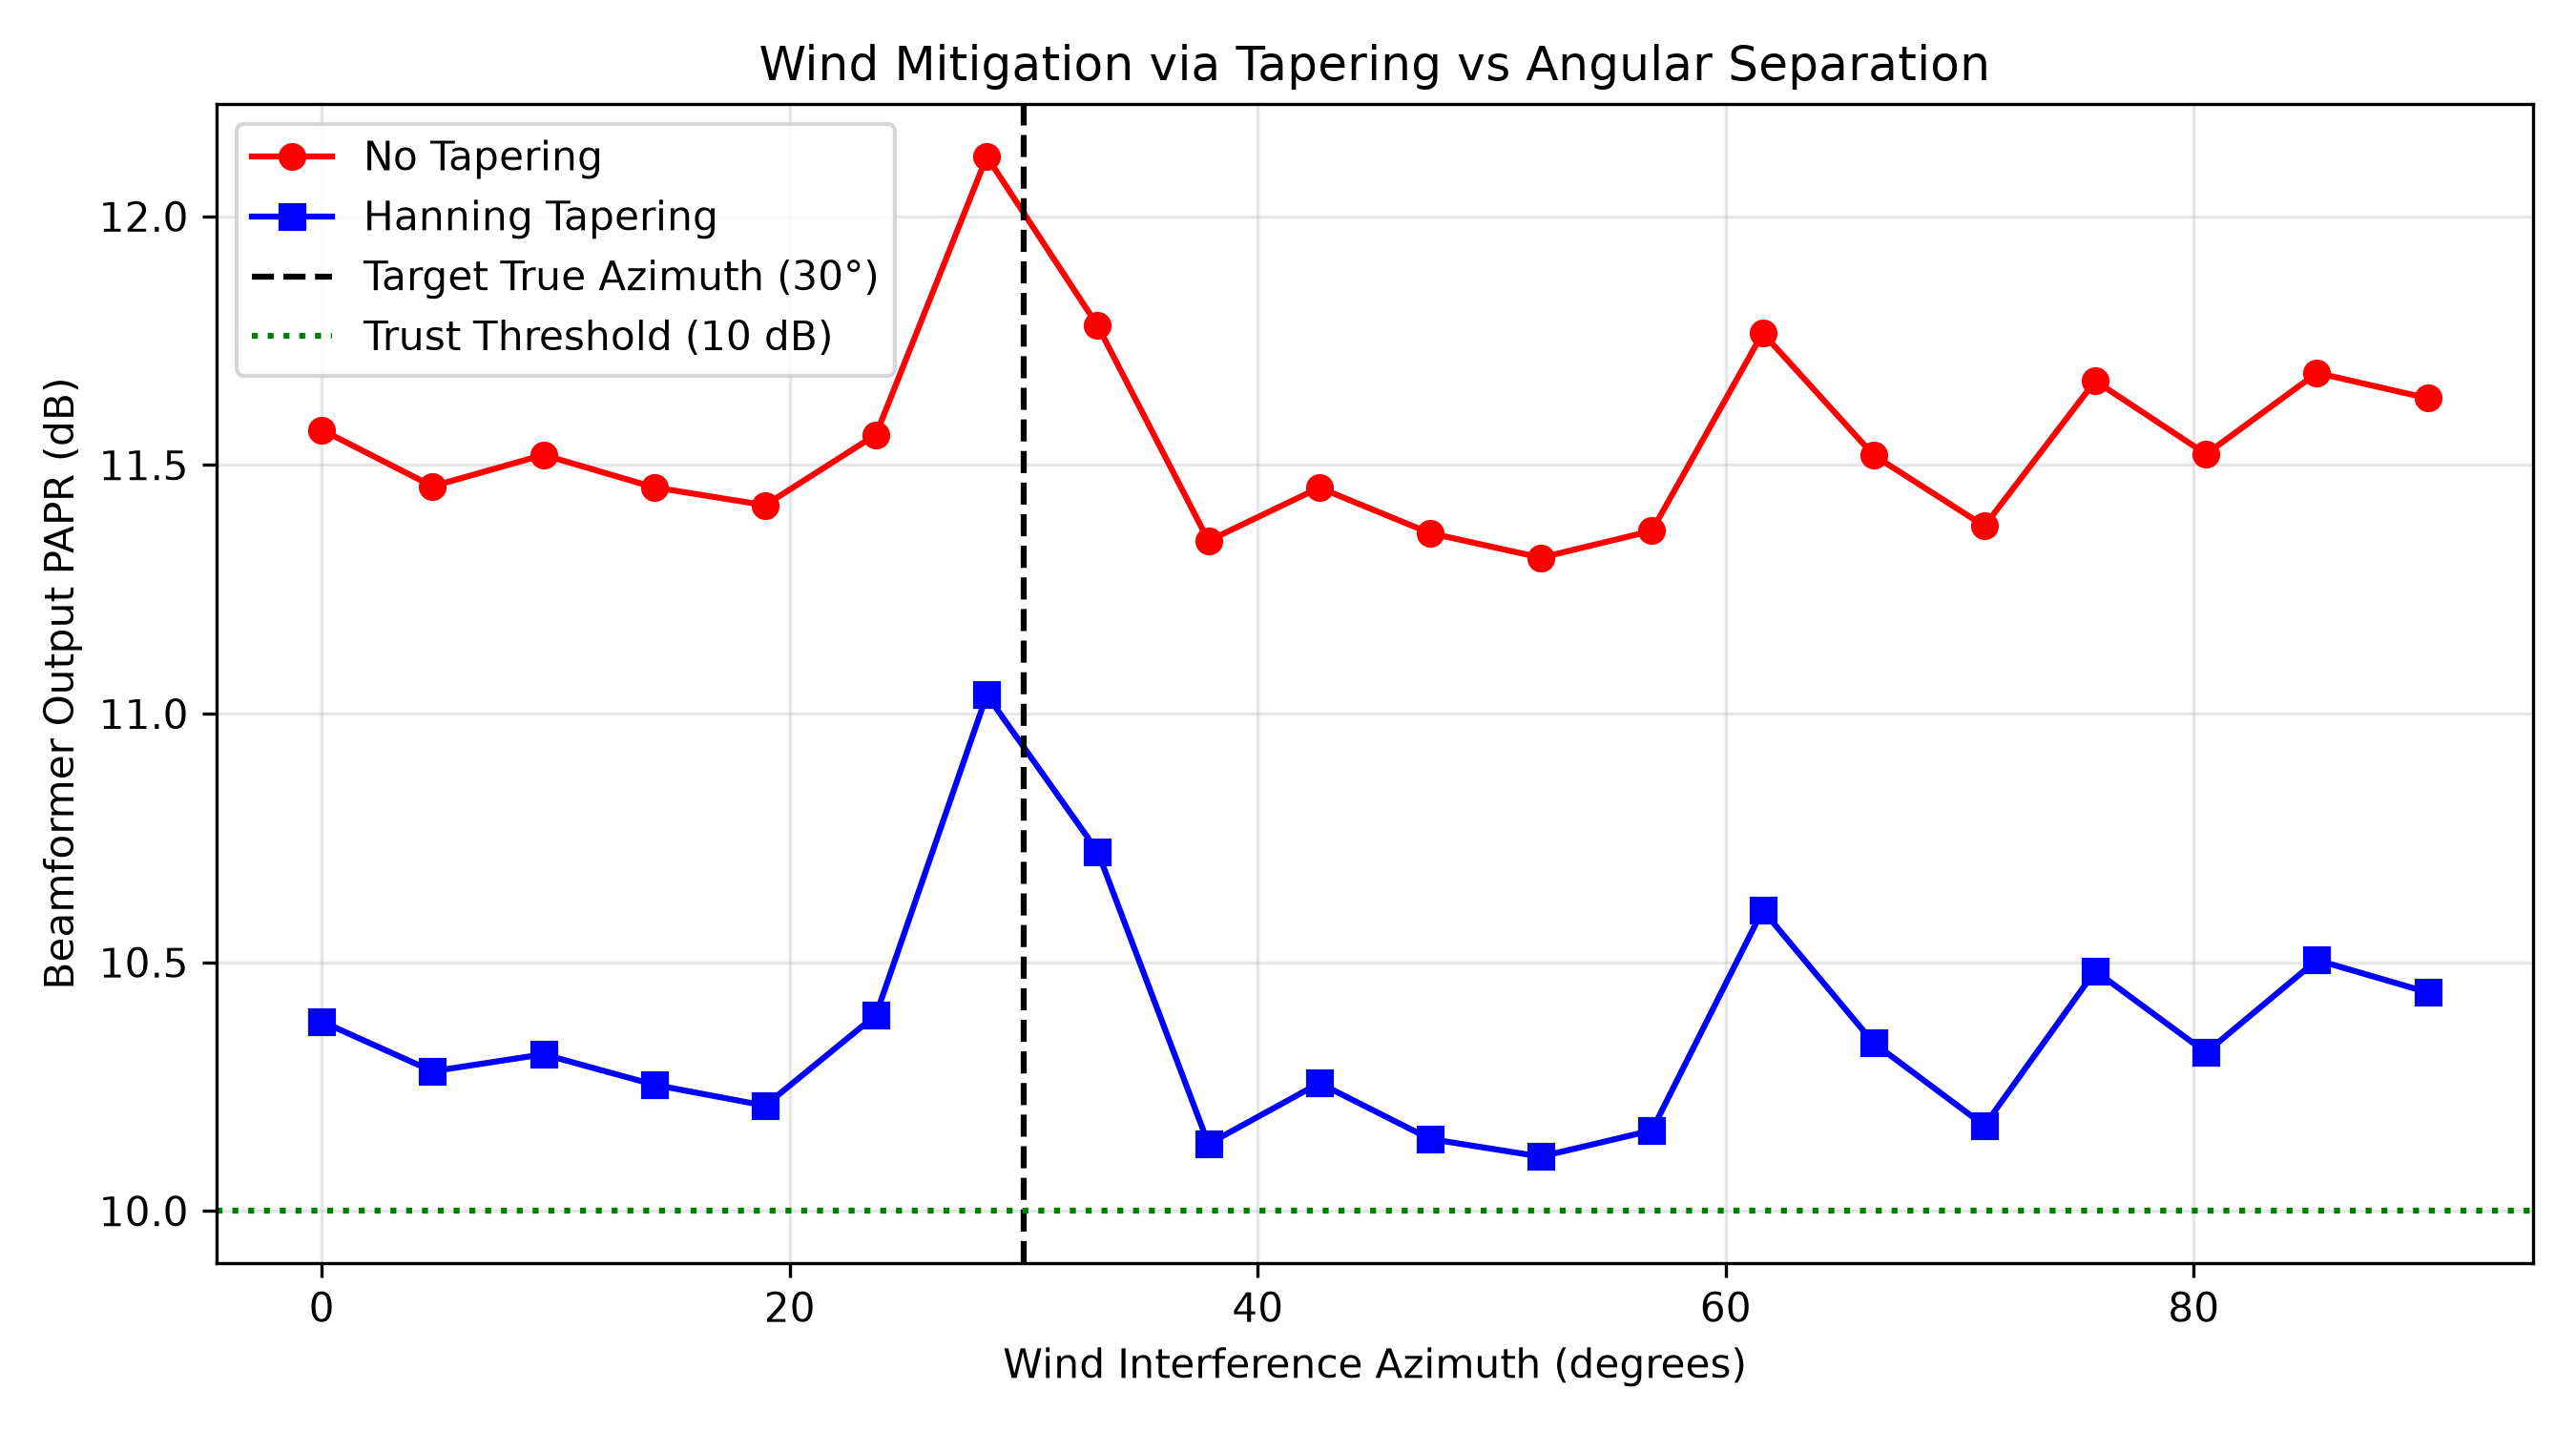
\includegraphics[width=0.8\textwidth]{figures/wind_tapering_scenario.png}
    \caption{PAPR of the target as intense wind sweeps past. The target is located at $30^\circ$.}
    \label{fig:wind}
\end{figure}

\subsection*{Operational Conclusions from Scenario 2}
\begin{itemize}
    \item \textbf{Direct Overlap ($20^\circ \to 40^\circ$):} If the wind blows directly from the target direction, \textbf{both} tapering and standard beamforming fail (PAPR crashes below $10$ dB). Tapering cannot defy physics if signals share the same spatial angle.
    \item \textbf{Angular Separation Recovery ($> 40^\circ$):} Once the wind separates from the target by more than $\approx 10^\circ$, Hanning tapering violently suppresses the wind sidelobes. Hanning recovers a trusted lock (PAPR $> 10$ dB) while the un-tapered array remains completely blind until the wind is $30^\circ$ away.
    \item \textbf{Takeaway:} Always engage Hanning tapering when operating in windy environments, provided the target is not flying directly downwind of the array.
\end{itemize}


\section{The Efficiency Matrix: Rivals vs. Complements}
You cannot manually inspect 300-point heatmaps in real-time. The pipeline implements three metrics: Spatial Coherence, PAPR, and Integrated Sidelobe Level (ISL). Are they rivals, or do they complement each other?

\begin{table}[h!]
    \centering
    \begin{tabularx}{\textwidth}{l l l X}
    \toprule
    \textbf{Metric} & \textbf{Cost} & \textbf{Role} & \textbf{Operational Action} \\
    \midrule
    \textbf{Coherence} & Low & Pre-filter & \textbf{Complements PAPR.} Computes in $<400$ms. If $< 0.1$, drop frame entirely. Saves 1.5 seconds of wasted CPU. \\
    \midrule
    \textbf{Map PAPR} & High & Lock Validator & \textbf{Primary Metric.} Validates the 2D output. If $> 10$ dB, the azimuth/elevation is trusted. \\
    \midrule
    \textbf{ISL} & High & Geometry Check & \textbf{Rival to PAPR.} ISL tells you if grating lobes exist, but PAPR inherently crashes if grating lobes dominate. For real-time targets, rely on PAPR and discard ISL to save code complexity. \\
    \bottomrule
    \end{tabularx}
    \caption{Metric Operational Action Matrix.}
\end{table}

\newpage
\appendix
\section{Appendix: Mathematical Definitions}
\textit{Included for technical verification, purposefully separated from executive conclusions.}

\subsection{Path Loss \& Log-Normal Shadowing}
The empirical path loss model incorporates geometric spreading, ISO 9613-1 absorption ($\alpha$), deterministic ground effects ($A_g$), and stochastic log-normal shadowing ($X_\sigma \sim \mathcal{N}(0, \sigma^2)$):
\begin{equation}
    PL(f, r) = 20\log_{10}(r) + \alpha(f)r + A_g + X_\sigma
\end{equation}

\subsection{Peak-to-Average Power Ratio (PAPR)}
\begin{equation}
    \text{PAPR (dB)} = 10\log_{10}\left( \frac{\max P(\theta, \phi)}{\frac{1}{K}\sum P(\theta, \phi)} \right)
\end{equation}
Where $K$ is the total number of evaluated steering angles in the search grid.

\end{document}
